\documentclass[a4paper,11pt, twocolumn]{article}
\usepackage[margin=0.8in]{geometry}
\usepackage{xcolor}
\usepackage{graphicx} %package to manage images
\graphicspath{ {./images/} }
\usepackage{float}
\usepackage{multicol}
\usepackage{tabularx}

\title{AS-2 Sequential Logic}
\author{Revision sheet}
\date{}

\usepackage{fancyhdr}
\pagestyle{fancy}
\fancyhead{} % clear all header fields
\renewcommand{\headrulewidth}{0pt} % no line in header area
\fancyfoot{} % clear all footer fields
\renewcommand{\footrulewidth}{0.4pt}
\fancyfoot[C]{\thepage} % page number in centre of the page
\fancyfoot[R]{\footnotesize Thomas Boxall \\ Images from the WJEC E-Book} % right hand footer has author name on top line and images reference on bottom line
\fancyfoot[L]{\footnotesize AS-2 Sequential Logic \\ Revision sheet} % left hand footer has title of document on top line and 'Revision Sheet' on bottom line


\begin{document}

\maketitle
\thispagestyle{fancy}

% CONTENTS OF THE REVISION SHEET HERE
\section{S-R Latch}
The set-reset latch has two inputs - $\overline{S}$ (Set) and $\overline{R}$ (Reset) and it has two outputs - $Q$ (Output) and $\overline{Q}$ (Inverted Output). The two inputs are active low which means that they need a low pulse to trigger. The S-R latch can be constructed from NAND gates.\\
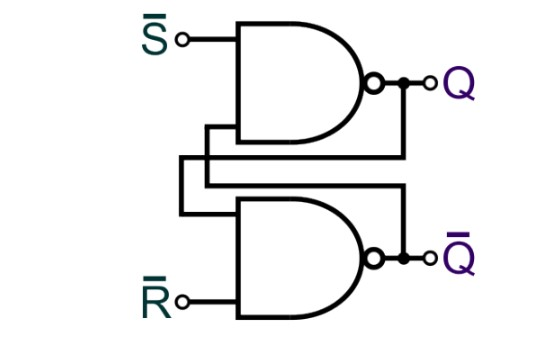
\includegraphics[width=0.45\textwidth]{srLatch.jpg}\\
The truth table for the circuit above is shown below. It has 4 states.
\begin{table}[H]
    \centering
    \begin{tabular}{l|cc|cc}
     & \multicolumn{2}{c}{Inputs} & \multicolumn{2}{c}{Outputs} \\
     & $\overline{S}$ & $\overline{R}$ & Q & $\overline{Q}$ \\
     \hline
    1 & 0 & 0 & 1 & 1 \\
    2 & 0 & 1 & 1 & 0 \\
    3 & 1 & 0 & 1 & 0 \\
    4 & 1 & 1 & 1 & 0
    \end{tabular}
\end{table}
\noindent As seen in the table above, there is an illegal state - when we press S and R (which makes both outputs 1). The timing diagram below shows the relationship between the inputs and outputs.
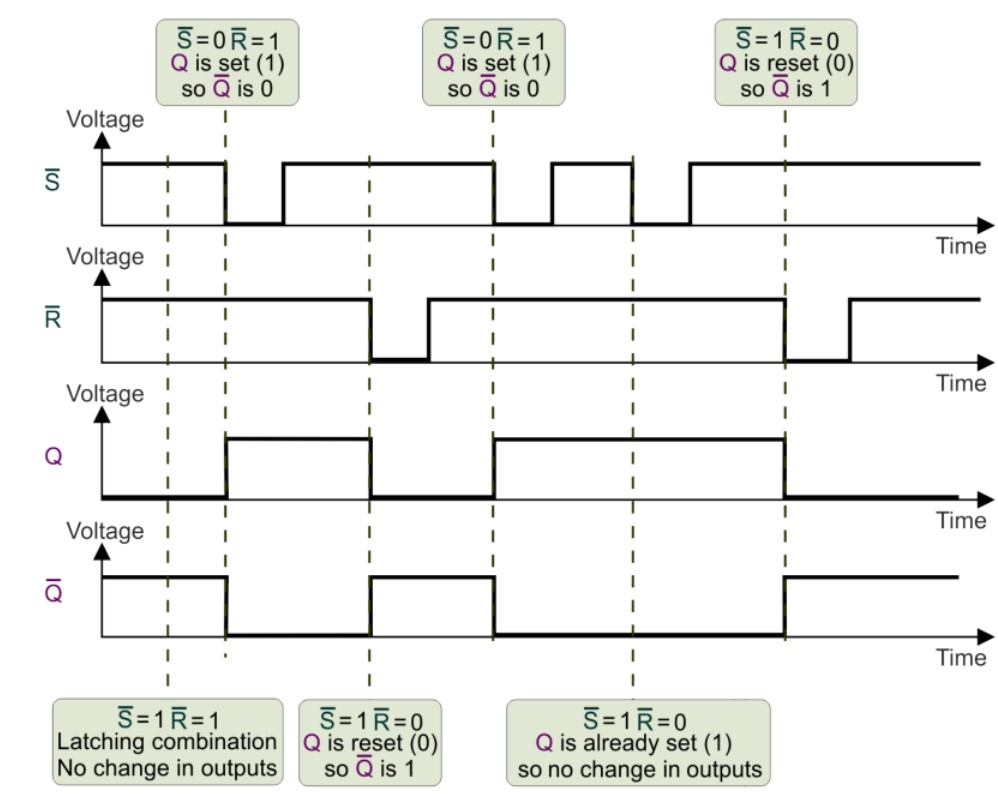
\includegraphics[width=0.45\textwidth]{srTiming.jpg}
\subsection{Uses Of The SR Latch}
The SR latch could be used for a bus stopping sign; keyless car ignition; wait light on road crossing; or to debounce a switch.
\subsection{Problems With The SR Latch}
It has an illegal state (when $\overline{S} = \overline{R} = 0$); the inputs are active low; and the outputs change immediately with inputs, often we want to synchronise changes to a clock pulse.
\subsection{Improvements To The SR Latch}
\subsubsection{Clocked SR Latch}
We can improve ths SR latch immediately, by adding another two NAND gates which allows for clock synchronisation of changes.\\
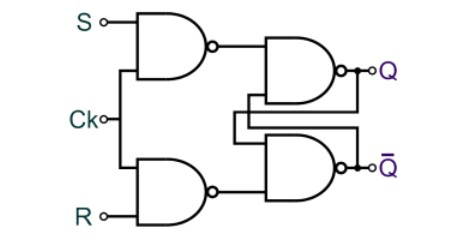
\includegraphics[width=0.45\textwidth]{srLatchClocked.jpg}\\
With this improved design, the flip flop can only change state when the clock (CK) is high and the inputs are active high. This is a good improvement, however there is still an illegal state. 
\subsubsection{Level Triggered D Flip-Flop}
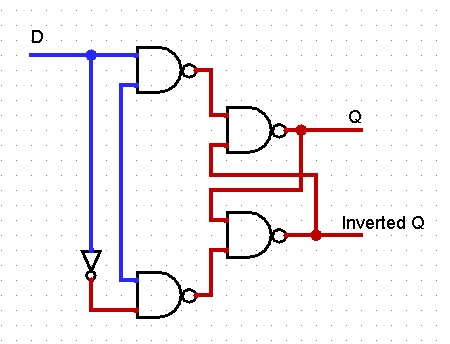
\includegraphics[width=0.45\textwidth]{levelTriggered.jpg}\\
In this iteration, S and R have been combined into one input ($D$). If D is logic high and the clock is logic high, the output is set and if D is logic low and the clock is logic high, the output is reset. This means that there is no illegal state.
\subsubsection{Edge Triggered D Flip-Flop}
This is shown further down the sheet, as it involves propagation delay.

\section{Propagation Delay}
Logic gates have a short delay between receiving an input and them changing their outputs. A transition gate can be used to detect a rising edge, as seen below.\\
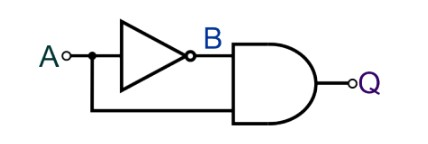
\includegraphics[width=0.45\textwidth]{transGate.jpg}\\
The relationship between the input, intermediary point (B) and output can be shown on a graph as follows.
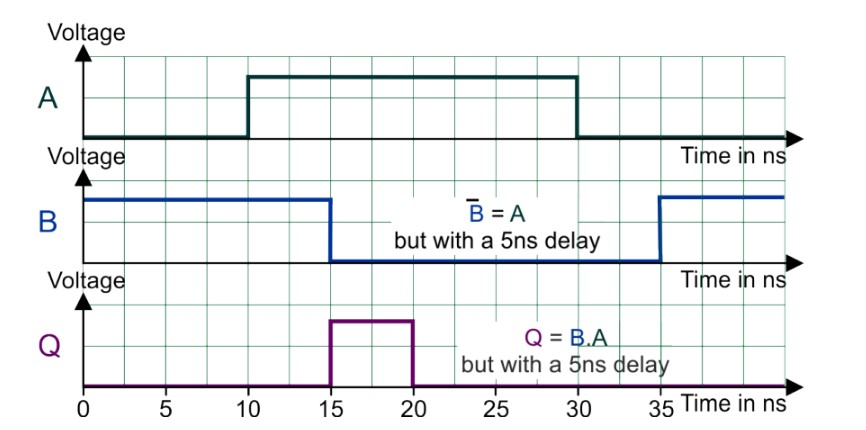
\includegraphics[width=0.45\textwidth]{transGateDiag.jpg}\\
The number of NOT gates used is variable, each with around 5 or 10ns delay.

\section{D-Type Flip-Flop}
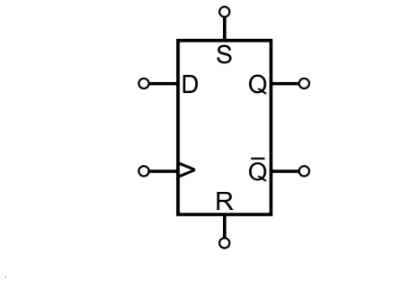
\includegraphics[width=0.45\textwidth]{dLatch.jpg}\\
Data is `clocked in' (sent to Q) on the rising edge of a clock pulse.
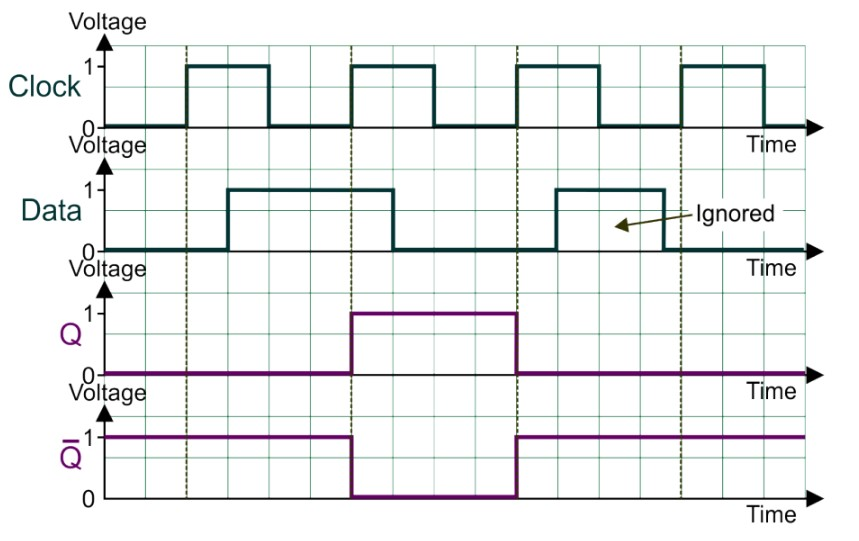
\includegraphics[width=0.45\textwidth]{dLatchDataQ.jpg}\\
S and R override the normal functioning of the D flip-flop, they change Q regardless of D or clock.
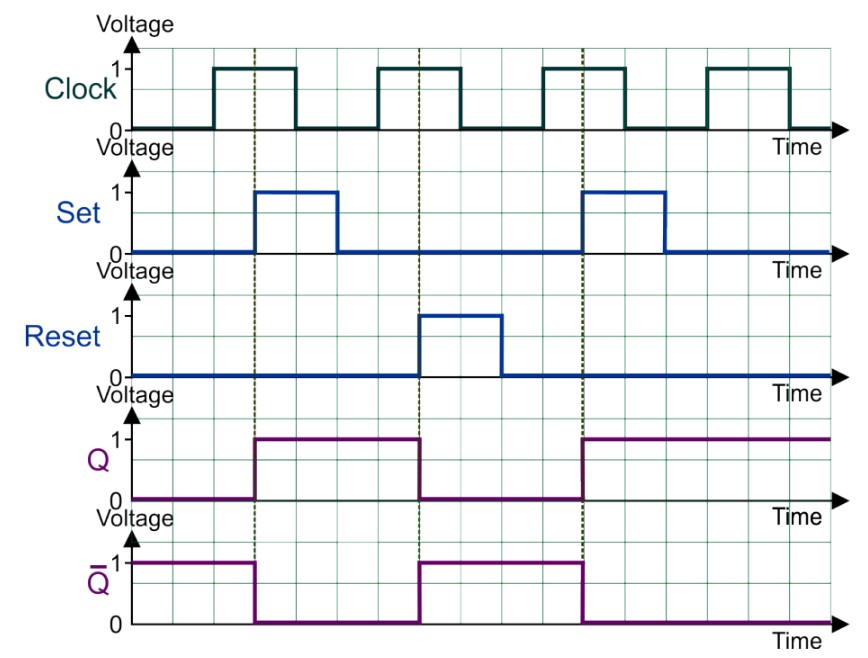
\includegraphics[width=0.45\textwidth]{dLatchSR.jpg}\\
Sometimes the Set and Reset inputs will be active low, this would be denoted either with a $\overline{S}$ or $\overline{R}$; or by a circle on the input, like the one on a NAND gate's output.

\section{Number Systems}
There are a number of different number systems and different methods to convert between them. 
\subsection{Denary (Base 10)}
Used most commonly, this is the one most people learn.
\begin{table}[H]
    \centering
    \begin{tabularx}{0.9\linewidth}{c c c c}
        1000 & 100 & 10 & 1 \\
        4 & 2 & 5 & 1
    \end{tabularx}
\end{table}
\noindent The total of the numbers above would be calculated in the following way:\\
$4251=(1000\times 4) + (100 \times 2) + (10 \times 5) + (1 \times 1)$\\
Denary is also known as base 10, this means each column can have one of ten possible values (0, 1, 2, 3, 4, 5, 6, 7, 8, 9)
\subsection{Binary (Base 2)}
This is base 2, this means each column can have one of two possible values (0, 1). The columns are also different. Moving from right to left, the columns double each time.
\begin{table}[H]
    \centering
    \begin{tabularx}{0.9\linewidth}{c c c c c c c c}
        128 & 64 & 32 & 16 & 8 & 4 & 2 & 1 \\
        1 & 0 & 1 & 1 & 0 & 0 & 1 & 1
    \end{tabularx}
\end{table}
\noindent The largest value which can be stored in binary is $11111111_2$ or $255_{10}$.
\subsection{Hexadecimal (Base 16)}
Also known as Hex. Using this method, numbers up to 255 can be stored in two characters. This is used a lot in computing, especially in graphics and website development. There are 16 columns (getting bigger in value from right to left)\\
F E D C B A 9 8 7 6 5 4 3 2 1 0 
\subsection{Converting Between Number Systems}
\subsubsection{Binary To Denary}
Add together all the columns in which there is a 1. Using the example shown in the binary section, the total would be 179.
\subsubsection{Denary To Binary}
This is the reverse of binary to denary. Work from right to left seeing if the value will fit into the column, if it won't then mark down an zero and move onto the next.
\subsubsection{Denary to Hex}
The easiest way to do this is to go via Binary. Convert the number into binary, then split the binary into two nibbles. The values inputted in the previous step don't need to change. With the two nibbles of (4, 2, 1, 0), convert each of them back into denary, giving two individual digits, then convert each of those into Hex. 

\section{Counters}
\subsection{1-Bit Counter}
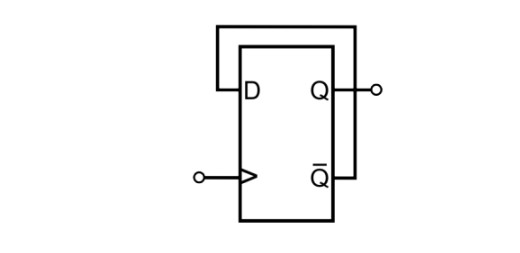
\includegraphics[width=0.45\textwidth]{1BitCounter.jpg}\\
On each rising edge of the clock, Q changes state. It counts from 0 to 1 then resets. This is the same circuit as used in a toggle flip flop (T Flip-Flop). It is a divide-by-two circuit, where the output frequency is half the input frequency.
\includegraphics[width=0.45\textwidth]{1BitCountergraph.jpg}
\subsection{2-Bit Counter}
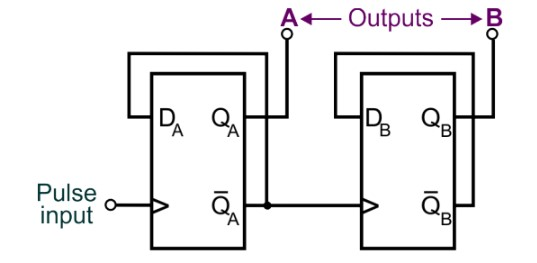
\includegraphics[width=0.45\textwidth]{2BitCounter.jpg}\\
The next counter along in the sequence is given a clock pulse on the rising edge of $\overline{Q}$ from the counter before it.
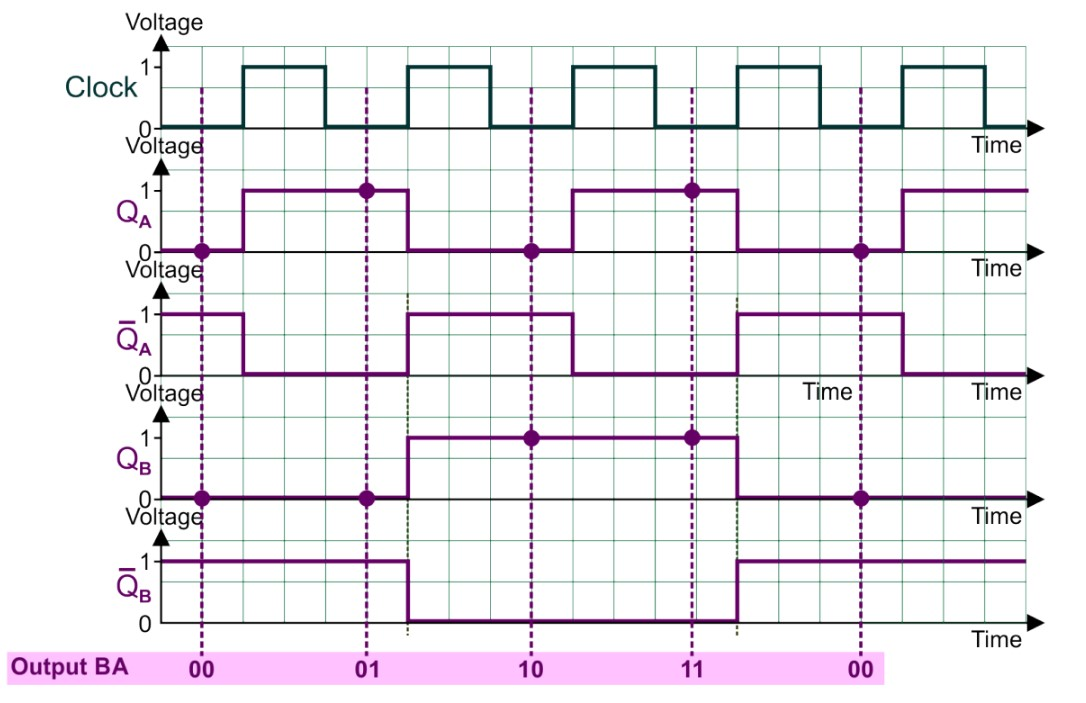
\includegraphics[width=0.45\textwidth]{2BitCounterGraph.jpg}\\
This gives us a scalable up-counter where the first flip flop to receive the clock forms the LSB and the last flip flop in the chain forms the MSB.
\subsection{Down Counters}
The circuit is basically the same apart from the clock pulse for the next counter comes from the Q output (rather than $\overline{Q}$) of the previous counter. 
\subsection{Counter ICs}
Chips are available to purchase which contain counters. These chips normally contain a 4-bit counter, which can be cascaded together to make a bigger counter. For example, shown below is a 8-bit counter (with a falling edge triggered clock).
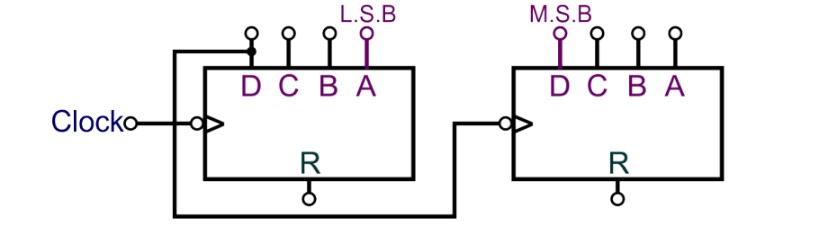
\includegraphics[width=0.45\textwidth]{8BitIC.jpg}
\subsection{BCD Counters}
\textit{Binary Coded Decimal} is a number system in which each decimal digit is represented by a 4-bit binary number from 0 to 9 (0000 to 1001). \\
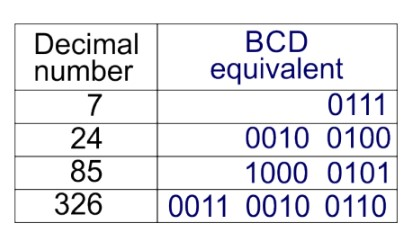
\includegraphics[width=0.45\textwidth]{bcdDecimal.jpg}\\
The table above shows some binary numbers in BCD. To convert a binary counter to a BCD counter, we use an AND gate on the D and B outputs (as this is 10, which is too high for BCD) then connect it to the reset of the counter. If the reset is active low, we can use the same connections, just with a NAND gate. 

\section{Seven Segment Displays}
These are used to display human-readable numbers. Usually, we'll use a `common cathode' display, this means all the cathodes of the LEDs are linked together, to a single ground pin. A decoder/driver is needed to convert from binary to seven-segment display format (these come as ICs). A current limiting resistor will also be needed for each segment as they are LEDs. The exact layouts of the pins vary from display to display.



\end{document}